\chapter{拼写与语音}
\label{chp:morph-phonology}

\begin{introduction}[章节要点]
  \item 古诺尔斯语的两种书写系统
  \item 古诺尔斯语字母的音值及单词拼读
  \item 音节划分规则
  \item 古诺尔斯语的音变
\end{introduction}

\section{书写系统和读音}
\label{sec:writing_system}

古诺尔斯语主要使用两种字母书写。其一是较早期的卢恩字母(Rune),后来则采用拉丁字母。最早发现的卢恩文字可追溯到公元2世纪。此时的古诺尔斯语尚处在非常原始的时期,故称为原始诺尔斯语。卢恩一词在日耳曼语中的意思是“秘密”,据神话记载,奥丁曾将自身作为祭品倒挂在世界之树上,在历经九夜的折磨后终于拾起了卢恩文字。这个神话的象征是奥丁通过苦行获得了智慧和奥义,因而卢恩的含义远不止一种书写系统那么简单。维京人认为卢恩可以用于占卜,到了中世纪晚期,北欧的文化已经受到了严重的基督教影响,其文字大量被拉丁化,卢恩字母丧失了日常沟通的功能,反而更加往神秘学的方向发展。

卢恩文字最初有24个,这套字母表称之为Elder Futhark,futhark是前六个字母的读音,和alphabet的含义(希腊字母表的前两个字母)类似。后来卢恩字母也发展出了16个字母的版本,称为Younger Futhark.
\begin{table}[H]
  \centering
  \caption*{\textbf{Elder Futhark} }
  \begin{tabular}{@{}llllllllllllllllllllllll@{}}
    \toprule
    \textarc{f} & \textarc{u} & \textarc{\th} & \textarc{a} & \textarc{r} & \textarc{k} & \textarc{g} & \textarc{w} & \textarc{h} & \textarc{n} & \textarc{i} & \textarc{j} & \textarc{p} & \textarc{I} & \textarc{R} & \textarc{s} & \textarc{t} & \textarc{b} & \textarc{e} & \textarc{m} & \textarc{l} & \textarc{\ng} & \textarc{d} & \textarc{o} \\ \midrule
    f           & u           & þ             & a           & r           & k           & g           & w           & h           & n           & i           & j           & p           & ï           & z           & s           & t           & b           & e           & m           & l           & ŋ             & d           & o           \\ \bottomrule
  \end{tabular}
\end{table}
\begin{table}[H]
  \centering
  \caption*{\textbf{Younger Futhark} }
  \begin{tabular}{@{}llllllllllllllll@{}}
    \toprule
    \textarm{f} & \textarm{u}                                              & \textarm{\th} & \textarn{\A} & \textarm{r} & \textarm{G} & \textarm{h} & \textarm{n}/\textarm{N} & \textarm{i} & \textarm{a} & \textarn{R} & \textarm{s}/\textarm{c} & \textarn{t} & \textarn{b} & \textarn{m} & \textarn{l} \\ \midrule
    f/v         & \begin{tabular}[c]{@{}l@{}}u/v/w,\\ y, o, ø\end{tabular} & þ, ð          & ą, o, æ      & r           & k, g, ŋ     & h           & n                       & e           & a, æ, e     & R           & s                       & t, d        & b, p        & m           & l           \\ \bottomrule
  \end{tabular}
\end{table}
卢恩文字或许有非常隐秘的作用,但这不在本书的讨论范围内。对于大部分中世纪的手稿而言,古诺尔斯语已经用上了我们熟悉的拉丁字母。

除了有最常见的26个字母外,古诺尔斯语的字母表中还包括几个特殊的辅音字母、元音字母和长音字母。这里我们只谈标准正字法下的字母,关于原始手稿中更复杂的情况,将在读本中进一步探索。

\begin{table}[H]
  \centering
  \begin{tabular}{@{}llll@{}}
    \toprule
    小写字母 & 大写字母 & 发音(国际音标) & 环境                     \\ \midrule
    á    & Á    & ɔː       &                        \\
    a    & A    & ɑ        &                        \\
    b    & B    & b        &                        \\
    c    & C    & k        &                        \\
    d    & D    & d        &                        \\
    ð    & Ð    & ð        &                        \\
    é    & É    & eː       &                        \\
    e    & E    & e        &                        \\
    f    & F    & (1) f    & 词首                     \\
         &      & (2) v    & 除词首外的其他位置              \\
    g    & G    & (1) g    & 词首,双写时,或在<gn>中         \\
         &      & (2) x    & 在<gs>或<gt>中            \\
         &      & (3) ɣ    & 在<gh>中                 \\
    h    & H    & h        &                        \\
    í    & Í    & iː       &                        \\
    i    & I    & i        &                        \\
    j    & J    & j        &                        \\
    k    & K    & (1)k     & 除了下面的情况                \\
         &      & (2)x     & 在<ks>或<kt>中            \\
    l    & L    & l        &                        \\
    m    & M    & m        &                        \\
    n    & N    & n        &                        \\
    ó    & Ó    & oː       &                        \\
    o    & O    & o        &                        \\
    p    & P    & (1) p    & 除了下面的情况                \\
         &      & (2) f    & <ps>或<pt>中             \\
    q    & Q    & k        & 总和u一起出现,qu和kv是一样的      \\
    r    & R    & r        &                        \\
    s    & S    & s        &                        \\
    t    & T    & t        &                        \\
    ú    & Ú    & uː       &                        \\
    u    & U    & u        &                        \\
    v    & V    & v        &                        \\
    w    & W    & w        &                        \\
    x    & X    & xs       &                        \\
    ý    & Ý    & yː       &                        \\
    y    & Y    & y        &                        \\
    z    & Z    & ts       & 极少出现,主要是-t/-d/-ð和-s的合写 \\
    þ    & Þ    & θ        &                        \\
    æ    & Æ    & ɛː       &                        \\
    ǫ́    & Ǫ́    & ɔː       &                        \\
    ǫ    & Ǫ    & ɔ        &                        \\
    ø    & Ø    & ø        &                        \\
    œ    & Œ    & øː       &                        \\ \bottomrule
  \end{tabular}
\end{table}

总体来说,古诺尔斯语有9个对立的基本元音音素,每个元音都有一个对应地长音。要构成长音,只需要在短音字母上添加锐音符`ˊ'。但有3个例外:
\begin{info}
  \begin{enumerate}
    \item a的长音á,在12世纪的古诺尔斯语已经与ǫ́合流,所以当时的音系中并没有一个长的a /ɑ:/。
    \item æ总是长元音,没有短元音与之对应 \footnotemark
          %!!!以下条目有字母缺失,须审阅!!!%
    \item ø的长元音是œ,一般不写†\'{ø}这种字母(但手稿中也有记载)。
  \end{enumerate}
\end{info}

\footnotetext{更早期的古诺尔斯语实际上有短的/ɛ/,这是a发生i-变异(参见 \ref{变元音} )的结果。}

这些音素,以及对应的字母在下表中标出,后面用尖括号<>标出的是这个元音的写法。关于前元音、后元音等术语,不熟悉的读者可以参照 \ref{变元音} 节中关于元音性质的描述。

\begin{table}[H]
  \centering
  \begin{tabular}{@{}ccccccccc@{}}
    \toprule
        & \multicolumn{4}{c}{\textbf{前元音}} & \multicolumn{4}{c}{\textbf{后元音}}                                                                                                \\ \cmidrule(l){2-9}
        & \multicolumn{2}{c}{非圆唇}          & \multicolumn{2}{c}{圆唇}           & \multicolumn{2}{c}{非圆唇} & \multicolumn{2}{c}{圆唇}                                             \\ \cmidrule(l){2-9}
    高元音 & i <i>                            & iː <í>                           & y <y>                   & yː <ý>                 &       &                  & u <u> & uː <ú> \\
    中元音 & e <e>                            & eː <é>                           & ø <ø>                   & øː <œ>                 &       &                  & o <o> & oː <ó> \\
    低元音 & ɛ                                & ɛː <æ>                           &                         &                        & a <a> & \textbackslash{} & ɔ <ǫ> & ɔː <ǫ́> \\ \bottomrule
  \end{tabular}
\end{table}

古诺尔斯语还有3个双元音/ɛi/, /ɔu/, /øy / 拼作 <ei>, <au>, <ey>.

低元音/ɛ/只出现在上述的双元音中。

古诺尔斯语的辅音比较规则,少数的例外一般表现为:

\begin{info}
  s/t之前的塞音会变成对应发音部位的清擦音。\footnotemark
\end{info}
\footnotetext{这个规律是原始语发生的日耳曼语擦音定律(Germanic spirant law)的残留。擦音定律和格林定律、维尔纳定律密切相关,涉及较为复杂的历史音变,请有兴趣的读者自查。}

古诺尔斯语的辅音也成对出现,双辅音与单辅音的区别仅在于前者的音值更长一些。j和v是半元音,它们的性质分别与i和u相似,在古诺尔斯语中经常发生音变(见 \ref{半元音的保持性} )。

\section{音节和重音}
\label{sec:accent}

音节是构成语音序列的单位,也是语音中最自然的语音结构单位。英文中的water就分为wa-和-ter两个音节。以英语为母语的人在拼读这个词的时候可能在t前停顿,但不可能在t后停顿,把water读成wat'er这样的形式。不同语言常有不同的音节划分规则,音节的类型也影响语言的韵律甚至是形态。

包括古诺尔斯语在内的大多数早期日耳曼语有复杂的音节划分模式,目前尚无一个统一的理论能够解释这些语言中的所有现象。语言学家主要从两个方面推测古代语言的音节划分,一是根据诗歌的规则;二是通过观察手稿中单词的记法。特别地,当一个单词出现在一行的末尾而恰好写不下时,这个词如何被拆分能够很好地反映它的音节情况。

就语法而言,古诺尔斯语的音节类型会影响部分动词(见 \ref{第一弱变位法} )和名词(见 \ref{ja-词干名词} )的变形,因此掌握音节的划分十分重要。有两种音节划分的方法可供参考,一种称为传统式,另一种称为格律式。如果读者之前没有接触过音韵学的知识,用传统式的划分已经可以很好地解决古诺尔斯语的问题(但通常这种方式和其他语言的音节划分不一样)。格律式划分和希腊语、拉丁语等划分一致,也更偏向于现代语音学的划分方法,因此介绍起来相对复杂些。

\subsection{传统式}

古诺尔斯语中有许多单音节词,例如á, til, at, rann. 单音节词只有一个元音,可以是长元音也可以是短元音。在多音节词中,如果这个词不是合成词,那么根据元音的位置划分音节(即非词首音节总以元音开头),例如far-a, kall-a, gǫrð-um, gam-all-a, hundr-að-a。在合成词中,根据组词的语素划分音节,例如vápn-lauss (< vápn + lauss, weapon-less), vík-ing-a-hǫfð-ing-i (< víkinga + hǫfðingi, Viking's chieftain). 由于元音和辅音有长短之分,音节也被分成以下四类:

\begin{table}[H]
  \centering
  \begin{tabular}{@{}cccc@{}}
    \toprule
    \multicolumn{2}{c}{\textbf{种类}} & \textbf{描述} & \textbf{举例}                  \\ \midrule
    1                               & 短           & 短元音+短辅音     & bað            \\
    2                               & 长           & 短元音+辅音簇     & rann, ǫnd      \\
    3                               & 长           & 长元音+短辅音/零辅音 & hús, fé, gnúa  \\
    4                               & 加长          & 长元音+辅音簇     & nótt,   blástr \\ \bottomrule
  \end{tabular}
\end{table}
其中,辅音簇(Consonant cluster)指的是多个辅音的集合。

\subsection{格律式}

格律式的划分方法与大多数音系学的理论一致,一个音节一般包括以下3个结构:
\begin{enumerate}
  \item 音节首(Onset)

        音节首总是由辅音充当。音节首可以是单辅音,也可以是多个辅音(辅音簇)。古诺尔斯语有些单音节词以元音开头,这时没有音节首。
  \item 音节核(Nucleus)

        音节核是一个响音,即可以是元音或者成音节的辅音。这是大多数语言的必有成分。
  \item 音节尾(Coda)

        由辅音充当,没有音节尾的音节是开音节,反之是闭音节。

\end{enumerate}

在这种划分下,上述的fara, kalla, gǫrðum, gamalla,hundraða就要重新划分为fa-ra, kal-la, gǫr-ðum, ga-mal-la, hun-dra-ða.细心的读者可能会想到面对词中的辅音簇时该如何划分?譬如是分成kal-la还是ka-lla?这个问题经常被讨论,但没有十分确切的定论。一般来说,有以下几个规则可供参考:

\begin{info}
  \begin{enumerate}
    \item 多音节词除了第一个音节外必有音节首。
    \item 多个辅音一般划分到两个音节。因而kal-la好于ka-lla.
    \item 规则1的例外是p,t,k,s和j,v,r一般划分到一个音节。因而si-tja好于sit-ja.
    \item 合成词在词素划分出区分一个音节。
  \end{enumerate}
\end{info}

按此法划分的音节按照音拍(Mora)的数量对其进行分类。音拍大致指的是语音中一个等时的单位。在古诺尔斯语中,音拍从音节核开始计算,音节首从不计入音拍。音节核和音节尾的音拍按下面的方式计算:

\begin{info}
  \begin{enumerate}
    \item 音节核中的单元音算一个音拍;双元音以及长元音算两个音拍。
    \item 音节尾如果是单辅音,不算音拍;如果有辅音簇,算一个音拍。
  \end{enumerate}
\end{info}

在这种划分下,音节可分为轻音节和重音节两种。轻音节只包括一个音拍,重音节则包括多个音拍:


\begin{table}[H]
  \centering
  \begin{tabular}{cll}
    \hline
    \textbf{种类}          & \textbf{音节核和音节尾可能的类型} & \textbf{举例}                                 \\ \hline
    \multirow{2}{*}{轻音节} & 1.短元音                 & \textbf{fa}-ra, \textbf{si}-tja             \\
                         & 2.短元音+单辅音             & \textbf{kal}-la, \textbf{bað}               \\[1ex]
    \multirow{2}{*}{重音节} & 1.短元音+辅音簇             & \textbf{rann}, \textbf{ungr}                \\
                         & 2.长/双元音+任意数量的辅音       & \textbf{hús}, \textbf{fé},  \textbf{blástr} \\ \hline
  \end{tabular}
\end{table}

一个例外情况是长元音+单辅音的组合在诗歌中被当作轻音节,例如búa,其中的成因尚不明确。

古诺尔斯语的重音落在第一个音节上。在两个语素的合成词中,一级重音落在第一个词的第一个音节上,第二个重音落在第二个词的第一个音节上(即总是落在词根上)。在三语素的合成词中,一级重音落在第一个词上,二级重音落在最后一个词上,三级重音落在中间词上,每个词的重音都遵循上述的规则。

重读音节中的元音是任意的,但在弱读音节中,只能是a, i, u这三个。弱读音节中经常发生元音的省略,详见 \ref{语音规则} 。

\section{变元音}
\label{变元音}

在古诺尔斯语的形态学中,变元音或者说元音变异(Umlaut)的现象是普遍存在的。变元音指的是两个元音同化的过程。具体来说,一个给定音节中元音的发音会因为说话者对下一个元音的预期而改变。由于这种预期,后面一个元音会影响到前面一个元音的发音,从而在本质上产生兼具两者特征的新元音。在古诺尔斯语中,i和u是最常见地引起这种音变的元音,因此把对应的过程分别称为i-变异和u-变异。

变元音的痕迹遍布整个古诺尔斯语的屈折系统,但变元音现象主要发生在原始诺尔斯语时期。读者必须认识到这个变化在用古诺尔斯语写作的时期之前已经发生完毕并且不再持续下去了。这就是说,并不是每个i或者u都会导致相应的变化,相反,i-变异和u-变异仅仅作为一种固定下来了的形态规则,保留在\textbf{\dotuline{部分的}}名词的变格和动词的变位中。一些符合变元音条件的地方可能并没有按预期的那样发生变元音,有些没有变元音发生条件的地方却反而没有变元音了。这两种现象都和古诺尔斯语的历史音变有关,而后者则尤其普遍,这主要是因为古诺尔斯语的词尾音节脱落得十分严重,许多本来能造成元音变异的音节在古诺尔斯语发展的过程中丢失了,只有其造成的变元音还保留下来。

变元音的本质是一种元音的同化现象。在介绍两种音变前,首先需要了解元音的一些基本理论。试着发i~a的音,会发现口腔逐渐打开,舌尖逐渐向口腔后部退缩,舌苔逐渐远离上颚。再试着发a~u的音,会发现口腔逐渐闭合,舌尖前后位置几乎不变,嘴唇逐渐收敛成o型。由此我们可以发现元音的性质至少和以下信息有关:舌尖位置,舌头最高处里上颚的距离,嘴型。根据发音时舌头在口腔中的相对位置,语言学家绘制了元音表:

\begin{figure}[H]
  \centering
  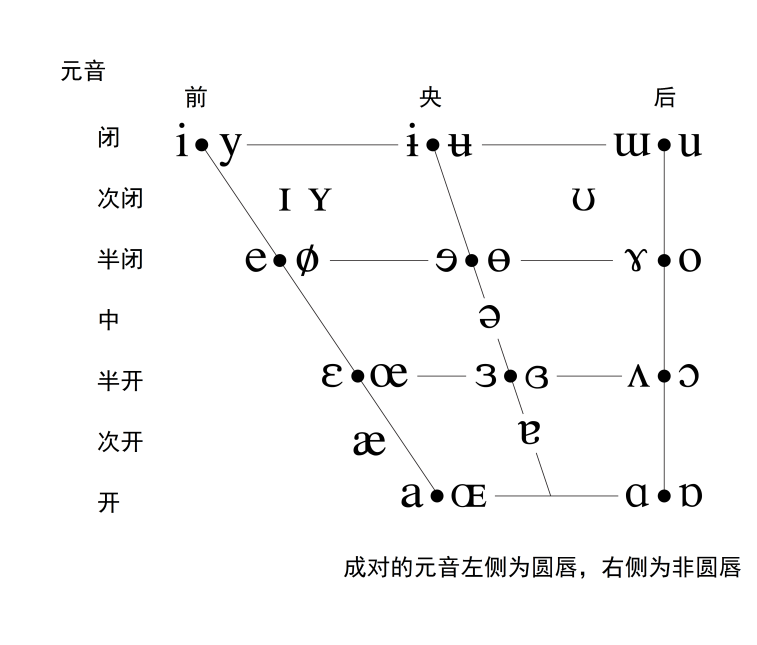
\includegraphics[width=0.5\linewidth]{Vowel_table.png}
\end{figure}

图表的纵轴称为元音高度,反映了舌头和口腔上部或两颚的距离;舌头位置较低的元音被放在元音图底部,而位置较高者则在元音图顶部。例如,{[}a{]}(相当于汉语拼音的``a'')被置于元音图下方,{[}i{]}(相当于汉语拼音的``i'')则被置于元音图上方。类似地,图表中的横轴称为元音舌位,反映了舌尖的前后位置;位置较靠前的元音被放在元音图左侧,而位置较靠后者则在元音图右侧。例如,{[}y{]}(相当于汉语拼音的``yu'')被置于元音图左方,{[}u{]}(相当于汉语拼音的``u'')则被置于元音图右方。当相同高度、舌位的元音成对出现时,右侧的是圆唇元音,左侧的则是非圆唇元音。发圆唇元音时,嘴唇形成一个圆形的开口,使嘴巴内侧的表面露出,如{[}y{]};而不圆唇元音发音时,嘴巴四周向后绷紧,嘴唇亦向后收缩,仅露出嘴唇的外部表面,如{[}i{]}。

一个元音的性质于是可以由三个维度表征:高度、舌位和圆唇度。元音高度区分高元音、低元音(或称闭元音、开元音);元音舌位区分前元音、后元音;圆唇度使得同一发音位置的元音总有圆唇元音和非圆唇元音的对立。

两种元音变异现象分别是:

1)i-变异。又叫前元音变异(Front mutation),指的是后一个音节中的i或j导致前一个音节中的元音舌位前移,高度抬升,但嘴型(圆唇/非圆唇)不改变的现象。由于i/j对应的是元音表中的前元音、高元音,i-变异就有把前一音节的元音向表中的左上角移动的倾向。

i-变异造成的效果是:
\begin{table}[H]
  \centering
  \begin{tabular}{cc}
    \hline
    \textbf{变化前} & \textbf{变化后} \\ \hline
    a            & e            \\
    á            & æ            \\
    o            & ø            \\
    ó            & œ            \\
    u            & y            \\
    ú            & ý            \\
    au           & ey           \\ \hline
  \end{tabular}
\end{table}

i-变异前后音长并不发生变化,因此变化后的元音也是成对的长短元音,但注意在12世纪的古诺尔斯语中,a和á的发音部位不同,e和æ的发音部位也略有区别。也有一些手稿把i-变异后的a写作ę,以区分其他的e,这个音最早应该读作/ɛ/,它是æ的短音。

以下情况中不发生i-变异:以i作为格标记的阳性中性名词(见 \ref{a/ja/wa-词干} )。i-变异失效的原因有很多:一种最简单的情况是原本的元音是*e,但在i-变异停止后才抬升为i;还有一种可能是,没有发生i-变异的词形被类推到了整个变形表中;但仍有一些问题无法解决。

2)u-变异。又叫唇化变异(Labial mutation),指的是后一个音节的u或v导致前一个音节中的元音被圆唇化,同时保持舌位不变。u-变异的效果是:

\begin{table}[H]
  \centering
  \begin{tabular}{cc}
    \hline
    \textbf{变化前} & \textbf{变化后} \\ \hline
    a            & ǫ            \\
    á            & (ǫ́) > á      \\
    非重读的a        & u            \\ \hline
  \end{tabular}
\end{table}

u-变异在古诺尔斯语的形态学中几乎只对a有效。但在其历史演变过程中,也造成了这样的音变:

\begin{table}[H]
  \centering
  \begin{tabular}{cc}
    \hline
    \textbf{变化前} & \textbf{变化后} \\ \hline
    e            & ø            \\
    é            & œ            \\
    i            & y            \\
    í            & ý            \\ \hline
  \end{tabular}
\end{table}

后一张表中的音变已经完全固定,即无论怎么添加含u的词尾,都不能再导致这样的变形了。只有在少量的词汇中可以看到这种这些音变保留的痕迹,例如英文``sing''的对应词†singva变成了古诺尔斯语的s\textbf{y}ng\textbf{v}a。

读者学习u-变异时,只需记住前一张表格中的内容,请注意,a在重读和非重读情况下造成的音变不同。长音的á由于性质特殊(回忆 \ref{sec:writing_system} 中元音的3个例外),在很早的时期就与ǫ́合流,以至于变元音的结果没有保留下来。

\section{语音规则}
\label{语音规则}

古诺尔斯语有一些规则的音变,下面将从元音和辅音两个方面进行说明。其中,辅音的规则音变相对更为普遍。

\subsection{元音的音变}
\label{元音的音变}

古诺尔斯语的共时系统中有下述的常见变化:
\subsubsection{元音变异}
\label{元音变异}


元音变异的原因和结果已经在 \ref{变元音} 节中详尽地阐释了,现在提供一些案例以供参考。

u-变异是一种比i-变异相对更``规则''的变化,许多造成u-音变的音节在古诺尔斯语中还保留了下来,但造成i-音变的音节大量脱落:

\begin{quote}
  arm + um > ormum `arms'

  sag + ur > sogur `stories'

  kall + að + u > kolluðu `called'
\end{quote}

请注意,ka\textsuperscript{[1]}lla\textsuperscript{[2]}ðu > kolluðu是一个连续的音变(在两个a上加了上标加以区别):词尾的-u首先造成非重读的a\textsuperscript{[2]}变成了u,这个u又为词根中的重读元音a\textsuperscript{[1]}提供了音变条件,这使得一个词中发生了两个u-音变,且结果不同。

i-变异有时发生的比较隐秘,试比较一个词干加上词尾后的结果,其中由*标出的词尾是古诺尔斯语的原始形式,但后来其中的元音脱落了:

\begin{quote}
  sat + ja > setja `set'

  vall + ir > vellir `fields'

  mús + *ir > mýss `mice'

  lát + *ir > lætr `lets'
\end{quote}


\subsubsection{元音省略和缩合}
\label{元音省略和缩合}

元音省略(Syncope)指的是非重读的短元音脱落的情况,最常造成语音省略的情况是:

\begin{info}
  \begin{enumerate}
    \item 弱读元音在辅音+元音前脱落。
    \item 以-i结尾的词干在与以元音开头的词尾接触时,i脱落。
  \end{enumerate}
\end{info}

常见的例子有:

\begin{quote}
  aptan + ar > aptnar `evenings'

  gamal + an > gamlan `old'

  komin + a > komna `come'

  lifi + um > lifum `live'
\end{quote}

元音缩合(Contraction)指的是一个非重读元音紧跟一个重读元音时发生的音变,如果两者都是前元音或者后元音(除了úa,óa,以及极少数情况下的 úu),就会合并为单个长音:

\begin{quote}
  tré + i > tré `tree'

  á + ar > ár `river'

  á + um > ám `rivers'

  trú + um > trúm `faithful'
\end{quote}

在前元音之前的后元音不发生音变,例如 búinn.在后元音之前的前元音经常形成双元音:

\begin{quote}
  fé + ar > fjár `cattle'

  kné + um > knjám/knjóm `knee'
\end{quote}

\subsubsection{元音延长或缩短}
\label{元音延长或缩短}

词尾的重读元音(开音节中)被延长,例如þú.当词尾的辅音脱落而导致原先处于中间位置的元音变成词尾元音时,规则同样成立,例如†vag > †va > vá.

辅音簇前的长元音常常被缩短,这种现象在双辅音前尤为明显。双元音ei缩短的结果是e,试比较下面一些词的原型和变格的形式:

\begin{quote}
  góðr --- gott `god'

  mín --- minn `my'

  heilagr --- helgan `holy'
\end{quote}

\begin{info}
  $\bullet$ \textbf{普罗科什定律(Prokosch's Law)}

  \indent
  为什么古诺尔斯语频繁地发生元音的延长和缩略?美国语言学家普罗科什(EduardProkosch)发现,古日耳曼语的音节有这样的规律(用格律划分法):

  \bigskip
  \indent
  \textbf{重音节有趋向2音拍的趋势;非重音节有趋向1音拍的趋势。}
  \bigskip

  \indent
  因此gott中的元音必须是短的,否则†gótt就有三个音拍了\footnotemark[3]。读者在记忆这一规则时,可以用普罗科什定律加以解释。
\end{info}

\footnotetext[1]{但是,这个规则也有例外,例如óðr  ---ótt.  类比这个词,góðr早期确实也有gótt的变形。普罗科什定律更类似于一种趋势而非一个必须遵守的规则。}

古诺尔斯语的元音系统还有一些值得关注的历史音变,这些音变基本发生在原始诺尔斯语时期,古诺尔斯语成文时已经停止,但这个音变的影响在许多词类中都有体现。

\subsubsection{元音分割}
\label{元音分割}

元音分割(Breaking)指的是特定环境下单元音变为双元音的过程。在古诺尔斯语中,唯一会发生这种音变的是来自原始诺尔斯语的*e. 元音分割的规则是:

\begin{info}
  \begin{enumerate}
    \item 如果下一个音节有a,则*e > ja;若下个音节有u,则*e > jǫ.
    \item 当*e紧跟在l, v, r后面时,元音分割不发生。
    \item 当jǫ后面有双辅音时,jǫ > jo.
  \end{enumerate}
\end{info}

元音分割造成了如下的结果:

\begin{quote}
  *herta > hjarta `heart'

  *skeldu > skjǫldu `shields'

  *brestaną > bresta `burst'

  *þekkuz > þjokkr `thick'
\end{quote}

这些变化在名词和动词的词根中都非常常见,但大多数词中元音分割贯穿了整个变形表,所以从共时层面来看,读者无法发现这一历史音变的痕迹。在有些词类中,特别是u-词干名词(见 \ref{u-词干} ),它们的词尾对应了不同的元音分割条件,使得某些形式中不发生元音分割,有的分割为ja,有的又分割为jǫ.

\subsubsection{抬升}
\label{抬升}

古诺尔斯语中常有e和i的交替,这一现象成因复杂。一方面,e > i的抬升可能是i-变异的影响;另一方面,在原始日耳曼语中也有抬升的痕迹。抬升的规则非常复杂,本书仅在发生这种现象的时候进行说明。

\subsection{辅音的音变}
\label{辅音的音变}

在某些情况下,辅音会发生规则的音变。最显著的几组如下所示,其中辅音同化的情况在古诺尔斯语中最为常见:

\subsubsection{辅音同化}
\label{辅音同化}

辅音同化指的是两个不同性质的辅音变成同一性质的音(经常造成双辅音),有五种重要的辅音同化现象:

\begin{enumerate}

  \item
        \phantomsection\label{_Ref117517668}{}-r 与前面的长音节中的 l, s或 n
        同化,由于-r是最常见的词尾之一,无论是动词、形容词还是名词中都能看到这一音变的痕迹:
        \begin{quote}
          sæl- + -r > sæll `happy'

          væn- + -r > vænn `hopeful'

          fús- + -r > fuss `willing'
        \end{quote}

  \item
        -ð-与前面的ð-同化为-dd-,与-t-或-s-同化为-tt-,
        -st-,-ð-是动词过去式的标记,这一现象亦非常常见,下面的例子都是动词和它的过去式形式:
        \begin{quote}
          eyða > eyddi `wasted'

          setja > setti `seated'

          kyssa > kyssti `kissed'

          kneikja > kneikti `bent';但merkja > merkði
          `marked'不发生同化
        \end{quote}

  \item
        齿音(-ð-/-d-/-n-)与后续的-t同化为-tt,这种情况通常发生简化变成单独的-t:
        \begin{quote}
          kald- + -t > kaltt > kalt `cold'

          harð- + -t > hartt > hart `hard'

          hin- + -t > hitt `the'
        \end{quote}


  \item
        -nn-有时在-r前变为-ð,这个变化最常见于两个非常基本的词中:
        \begin{quote}
          mann- + -r > maðr `man'

          ann(a)r- + -ar > aðrar `another'
        \end{quote}

  \item
        -k-+
        -ð-有时同化为-tt-,但有时也变成-kt-,还有时不发生改变。这些音变都发生在过去式中,造成这种交替的很可能是类比的结果:
        \begin{quote}
          sœkja > sótti `sought'

          þykkja > þótti `thought'

          kneikja > kneikti `bent'

          但merkja > merkði `marked'不发生同化
        \end{quote}
\end{enumerate}


\subsubsection{词尾清化}
\label{词尾清化}

结尾的辅音簇先清化,有时还进一步发生同化,主要出现在部分强动词的过去式中,这些音变包括-nd
> -nt > -tt; -ng > -nk
> -kk; -ld > -lt:

\begin{quote}
  binda > batt `bound'

  stinga > stakk `stung'

  gjalda > galt `paid'

  ganga > gekk `went'

  halda > helt `held'
\end{quote}

\subsubsection{辅音脱落}
\label{辅音脱落}

非重读音节中的-n-或-l-有时在词尾的-t前脱落:

\begin{quote}
  mikil- + -t > mikit `large'

  búin- + -t > búit `lived'

  但gamal- + -t > gamalt `old'不变
\end{quote}

\subsubsection{辅音延长}
\label{辅音延长}

词尾的-t或-r加在长元音词干后会拖长一拍,请注意这和前述的普罗科什定律有区别,前者通常适用于CV:C型词干,而这里属于CV:型词干,这种情况下并不造成元音的缩短。这种辅音延长更可能是受到前面的长元音的影响,如果长元音缩短,这种音变的条件就消失了:

\begin{quote}
  ný- + -t > nýtt `new'

  fá- + -ri> fárri `few'
\end{quote}

\subsubsection{辅音简化}
\label{辅音简化}
辅音簇后接辅音时,如果形成了双辅音,则双辅音简化为单辅音:

\begin{quote}
  akr- + -r > *akrr > akr `meadow'

  fagr- + -rar > *fagrrar > fagrar `fair'

  jarl- + -r > *jarll > jarl `noble'
\end{quote}

\subsection{半元音的保持性}
\label{半元音的保持性}

古诺尔斯语有两个半元音j和v,这两个半元音的由来涉及到比较复杂的历史音变,在古诺尔斯语中,半元音经常发生脱落。本节首先介绍几个共时系统中的规则,然后提供一些简单的历时规律以供读者进一步参考。

在共时系统中,半元音的遵循的总体规则是:

\begin{info}
  \begin{enumerate}
    \item 半元音在音质``相近''的元音前脱落,在音质``相异''的元音前保留。
    \item j在出现在后元音(a, o, u, ǫ及其长音)前;
    \item v出现在非圆唇元音(i, e, a及其长音、æ)前(但有例外ǫ和ó)。
  \end{enumerate}
\end{info}

根据这个规律,在任何情况下,类似于†ji或†vu的形式是不允许出现的,动词系统中经常涉及元音的变化,所以半元音常消失:

\begin{quote}
  krjúp + *ir > *krjýpr > krýpr `crawls'

  *vurðu > urðu `became'
\end{quote}

许多动词、名词的词干尾保留了一个半元音,这里的半元音不仅要遵守上述的规则,而且还在辅音词尾或者零词尾(即不加任何词尾)前脱落,即:

\begin{info}
  词干尾的半元音只可能保留在以音质``相异''的元音开头的词尾前。
\end{info}

\begin{quote}
  deyj- + -r > deyr `dies'

  telj- + -i > teli `would tell'

  verj- + -um > verjum `defended'

  songv + Ø > song `song'

  hoggv + um > hoggum `strike'

  sæv- + -ar > sævar `strike'
\end{quote}

古诺尔斯语的j和v曾经发生了历史性的脱落,这主要表现为:

1.
在词首,j全部脱落;v在l或者r前脱落。古诺尔斯语词首的j全部由元音分割而来,比较几个古诺尔斯语和英语的同源词:

\begin{quote}
  ungr------\textbf{y}oung (j脱落)

  \textbf{ja}fn------\textbf{e}ven (元音分割)

  ríta------\textbf{wr}ite (v脱落)
\end{quote}

2. 在词中,w在ó和ú之后脱落:

\begin{quote}
  glóa------glo\textbf{w}
\end{quote}






